%xelatex -shell-escape -output-directory=bin ergasia.tex
\documentclass{assignment}

\usepackage{enumerate} % Για την χρησιμοποίηση roman enumerate
\usepackage{pdflscape}

%\university{Πανεπιστήμιο Πειραιώς}{Πα.Πει.}
%\school{Τμήμα Πληροφορικής}{Π.Μ.Σ. "Πληροφορική"}
%\department{Πρόγραμμα Μεταπτυχιακών Σπουδών «Πληροφορική»}{}
%\cover{images/cover.jpg}{http://www.cyberciti.biz/faq/grub-boot-into-single-user-mode/}

\title{Βάσεις Δεδομένων \\ Εργασία Εξαμήνου}
%\projectlevel{Εργαστήριο Λειτουργικά Συστήματα}
%\lesson{Λειτουργικά Συστήματα}{1}
\date{Αθήνα, 2014}

\author{Αναγνωστόπουλος Βασίλης - Θάνος}
%\register{ΜΠΠΛ13002}{1}

%\exercauthor{Αναγνωστόπουλος Βασίλης - Θάνος}{06107083}{9}

%\advisor{Τσακίρη Μαρία, Αναπληρώτρια Καθηγήτρια Ε.Μ.Π.}

\begin{document}

\maketitle
% Να σκεφτώ τί αλλαγές θέλω να κάνω με τις αριθμήσεις και άμα θέλω να κάνω.
% Να σκεφτώ να τις ενσωματώσω και στο assignment.cls

\setcounter{page}{1} 
\pagenumbering{roman}

\pagestyle{plain}
\tableofcontents
\newpage


%\pagestyle{headings}
%\pagestyle{fancy}
\setcounter{page}{1} 
\pagenumbering{arabic}

\section{Εισαγωγή - Αντικείμενο της άσκησης}

Σκοπός της άσκησης είναι η σχεδίαση και υλοποίηση μιας βάσης δεδομένων,
ακολουθώντας τη μεθοδολογία υλοποίησης βάσεων δεδομένων. Τόσο το περιεχόμενο όσο και οι απαιτήσεις της βάσης δεδομένων που θα
υλοποιηθεί θα στηρίζονται σε πραγματικά δεδομένα. Το ΣΔΒΔ στο οποίο θα υλοποιηθεί η βάση δεδομένων θα είναι αυτό της MySQL.

\subsection{Μεθοδολογία υλοποίησης της άσκησης}

Στα πλαίσια της εργασίας θα ακολουθηθούν τα εξής βήματα:

\begin{description}

  \item [Βήμα 1: Ανάλυση απαιτήσεων.]  Θα επιλεχθούν δεδομένα μίας ορισμένης θεματολογίας. Τα δεδομένα αυτά τα παρέχει ένας πελάτης και αυτά έμμεσα υποδηλώνουν τις απαιτήσεις της βάσης δεδομένων. Μέσα από την ανάλυση αυτή θα αποσαφηνιστούν οι περιορισμοί της προς υλοποίησης βάσης δεδομένων. Το πρώτο βήμα παίζει σπουδαίο ρόλο στην πορεία του σχεδιασμού της βάσης δεδομένων, αφού λανθασμένη εκτίμηση των απαιτήσεων οδηγεί σε διαφορετικούς προορισμούς, άρα λανθασμένο σχεδιασμό. 

  \item [Βήμα 2: Σχεδιασμός και υλοποίησης της Βάσης Δεδομένων.] Μέσα στο βήμα διακρίνονται 3 φάσεις:

  \begin{itemize}

    \item Η α` φάση (εννοιολογικός σχεδιασμός) περιλαμβάνει τη δημιουργία ενός εννοιολογικού σχήματος για τη βάση δεδομένων, με χρήση ενός εννοιολογικού μοντέλου δεδομένων υψηλού επιπέδου. Το εννοιολογικό σχήμα είναι μια περιεκτική περιγραφή των απαιτήσεων (ή τουλάχιστον των περισσότερων από τις απαιτήσεις) των χρηστών σχετικά με τα δεδομένα και περιλαμβάνει 2 λεπτομερείς περιγραφές των τύπων δεδομένων, των συσχετίσεων και των περιορισμών. Για τον εννοιολογικό σχεδιασμό της βάσης δεδομένων της εφαρμογής που θα αναπτύξετε, θα χρησιμοποιηθεί το μοντέλο Οντοτήτων - Συσχετίσεων (\en{Entity - Relationship Model}).

    \item Η β` φάση (λογικός σχεδιασμός) περιλαμβάνει τη δημιουργία ενός λογικού σχήματος για τη βάση δεδομένων, με χρήση ενός λογικού μοντέλου δεδομένων, συγκεκριμένα του Σχεσιακού Μοντέλου (\en{Relational Model}). Το λογικό σχήμα που θα παραχθεί στη δεύτερη φάση πρέπει να είναι συμβατό με το εννοιολογικό σχήμα της πρώτης φάσης και να προκύψει από αυτό μετά από κατάλληλους μετασχηματισμούς.

    \item Η γ` φάση (υλοποίηση) περιλαμβάνει την υλοποίηση του σχεσιακού σχήματος της δεύτερης φάσης στο ΣΔΒΔ που θα έχει επιλεγεί καθώς και τη φόρτωση της βάσης δεδομένων με ενδεικτικά (πραγματικά ή ρεαλιστικά) δεδομένα.

  \end{itemize}

\end{description}

\subsection{Παραδοτέα}

\begin{enumerate}

  \item εκτυπωμένη αναφορά στην οποία θα περιγράφονται λεπτομερώς τα βήματα 1 - 2 της εργασίας. Συγκεκριμένα θα περιγράφονται λεπτομερώς:

  \begin{enumerate}[i]
    \item Προδιαγραφές της βάσης δεδομένων σε μορφή ελεύθερου κειμένου (Βήμα 1)
    \item Εννοιολογικό σχήμα της βάσης δεδομένων σε μορφή ER (Βήμα 2α) + λίστα απαιτήσεων που δεν μπόρεσαν να απεικονιστούν στο διάγραμμα ER
    \item Σχεσιακό σχήμα της βάσης δεδομένων σε γραφική μορφή (Βήμα 2β)
    \item Σχεσιακό σχήμα της βάσης δεδομένων σε μορφή SQL script και ενδεικτικά \en{screenshots} με καταχωρημένα δεδομένα (Βήμα 2γ)
  \end{enumerate}

  \item CD με την αναφορά σε ηλεκτρονική μορφή καθώς και αρχείο \en{bakcup / export} της βάσης δεδομένων που προέκυψε από το βήμα 2.

\end{enumerate}

\section{Ανάλυση απαιτήσεων}

Η ανάλυση απαιτήσεων περιλαμβάνει τις εργασίες για τον καθορισμό των αναγκών ή των προϋποθέσεων που χρειάζονται για την ολοκλήρωση ενός προϊόντος (στην συγκεκριμένη περίπτωση της βάσης δεδομένων μας). Στην ανάλυση απαιτήσεων λαμβάνονται υπόψιν οι ενδεχόμενες αντικρουόμενες απαιτήσεις των διαφόρων μερών ενώ ταυτόχρονα αναλύονται και τεκμηριώνονται οι τυχόν απαιτήσεις του προϊόντος \cite{wiki:requirement_analysis}. Για να είναι επιτυχές ένα σύστημα βάσεως δεδομένων θα πρέπει να είναι προσαρμοσμένο στις ανάγκες, απαιτήσεις, αλλά και προσδοκίες του τελικού χρήστη. Αυτό σημαίνει ότι το ζητούμενο είναι, τί πραγματικά επιθυμεί ο χρήστης, τί ακριβώς περιμένει από το σύστημα και πόσο φιλικό είναι αυτό σε αυτόν και κατά πόσο ικανοποιεί τους σκοπούς για τους οποίους υλοποιήθηκε.

%\subsection{Σκοπός δημιουργίας της βάσης δεδομένων}

Σκοπός της συγκεκριμένης βάσης δεδομένων είναι η ταξινόμηση των βιβλίων (είτε αυτά είναι σε φυσική ή ηλεκτρονική μορφή) που έχουν μία ομάδα χρηστών, έτσι ώστε να είναι δυνατή η γρήγορη εύρεση ενός βιβλίου με βάση κάποια κριτήρια. 

Τα ερωτήματα σε αρχικό στάδιο που θα απαντά η βάση είναι τα παρακάτω:
\begin{itemize}
  \item Τι βιβλία υπάρχουν στην κατοχή των χρηστών
  \item Τι βιβλία έχει ο κάθε χρήστης και ποια είναι η μορφή τους
  \item Τι βιβλία ένας συγγραφέας (ή ένας εκδότης) έχει γράψει (ή έχει εκδώσει)
\end{itemize}

%\emph{Χρειάζεται να αναφέρω τίποτα άλλο στην ανάλυση απαιτήσεων;}
%\subsection{Πληροφορίες που απαιτούνται}


%\subsection{Κατηγορίες χρηστών βάσης δεδομένων}

%Χρήστες μίας βάσης δεδομένων είναι όσοι χρησιμοποιούν την βάση δεδομένων είτε για την απόκτηση πληροφορίας είτε για συντήρηση της βάσης δεδομένων \cite{baseis_eap}.

\section{Σχεδιασμός και υλοποίησης της Βάσης Δεδομένων}

Σχεδιασμός είναι η διαδικασία δημιουργίας του σχήματος (\en{schema}) της βάσης δεδομένων χρησιμοποιώντας ένα επιλεγμένο Μοντέλο \cite{class_notes}.

Σε αυτή την ενότητα αναλύονται οι παραδοχές και οι αποφάσεις που πάρθηκαν κατά την διάρκεια σχεδίασης του βάσης δεδομένων.

\subsection{Εννοιολογικός σχεδιασμός}

Για τον εννοιολογικό σχεδιασμό της βάσης δεδομένων θα χρησιμοποιηθεί το μοντέλο Οντοτήτων - Συσχετίσεων.  Στην τεχνολογία λογισμικού, το μοντέλο οντοτήτων - συσχετίσεων (\en{entity–relationship model (ER model)}) είναι ένα απλό, σαφές, αφαιρετικό, ιδεατό, μοντέλο δεδομένων, τα οποία έχουν καθορισμένη δομή και στηρίζονται στο γραφικό συμβολισμό. Χρησιμοποιείται για να παρέχει ένα εννοιολογικό σχήμα κατά τη σχεδίαση βάσεων δεδομένων, ως μοντέλο δεδομένων ενός συστήματος και των απαιτήσεών του με \en{top-down} προσέγγιση \cite{wiki:Entity_relationship_model, class_notes}.

Σε αυτή την ενότητα θα γίνει καταγραφή των Οντοτήτων της βάσης δεδομένων καθώς και των μεταξύ τους συσχετίσεων.

Υπάρχουν δύο βασικές εννοιολογικές έννοιες \cite{class_notes}:
\begin{description}
  \item[Οντότητες (\en{entities}):] Συγκεκριμένα αντικείμενα που υπάρχουν (ή πιστεύεται ότι υπάρχουν) και μπορούν να αναπαρασταθούν στην βάση δεδομένων. Οι οντότητες μπορούν να έχουν χαρακτηριστικά (\en{attributes}) που είναι ιδιότητες που τα χαρακτηρίζουν
  \item[Συσχετίσεις (\en{relationships}):] Είναι επίσης (ειδικά) αντικείμενα που αντιστοιχούν δύο ή περισσότερες ξεχωριστές οντότητες με ένα συγκεκριμένο νόημα (τυπικά, μια Συσχέτιση είναι ένα διατεταγμένο σύνολο οντοτήτων). Ομοίως και οι συσχετίσεις μπορούν να έχουν χαρακτηριστικά.
\end{description}

Σκοπός της συγκεκριμένης βάσης δεδομένων είναι η καταγραφή και ταξινόμηση όλων των βιβλίων των χρηστών. Επομένως δύο οντότητες οι οποίες θα πρέπει να υπάρχουν στην βάση δεδομένων είναι τα βιβλία καθώς και οι χρήστης (με όποια τυχόν χαρακτηριστικά χρειάζονται να καταγράφονται ακόμα για αυτές τις δύο οντότητες).

Συγκεκριμένα για τα βιβλία θα καταγράφεται ακόμα ο τίτλος του, η γλώσσα στην οποία είναι γραμμένο που είναι πλείοτιμο χαρακτηριστικό, μία περιγραφή για το βιβλίο και τα αναγνωριστικά των βιβλίων (π.χ. isbn, google books number, κ.λ.π.) τα οποία είναι πλειότιμα και σύνθετα χαρακτηριστικά. Ακόμα θα υπάρχει εξειδίκευση μεταξύ των έντυπων βιβλίων και των βιβλίων τα οποία είναι σε ηλεκτρονική μορφή. Στα μεν έντυπα θα καταγράφεται και η φυσική τους τοποθεσία, ενώ στα ηλεκτρονικά βιβλία θα καταγράφεται και τα δεδομένα τους (δηλαδή σε τί μορφή είναι αποθηκευμένα και το όνομα του αρχείου)

Για τους χρήστες θα καταγράφουμε μόνο το όνομα τους.

Ακόμα κάθε βιβλίο έχει ένα τουλάχιστον συγγραφέα καθώς και έναν εκδότη. Επομένως αυτά θα γίνουν ομοίως οντότητες στο διάγραμμα μας.

Τέλος θα υπάρχουν ακόμα και ετικέτες οι οποίες θα είναι διαφορετικές ανάλογα το βιβλίο και τον χρήστη. Οι ετικέτες θα γίνουν ξεχωριστές οντότητες και θα συνδέονται ταυτόχρονα με τα βιβλία και τους χρήστες.

Όλα τα παραπάνω συνοψίζονται στο σχήμα \ref{fig:ER:diagram}.

%Τα indetifiers είναι πλειότιμα χαρακτηριστικά (έχει πολλαπλές τιμές)

%Η πληθικότητα (\en{cardinality}) ενός τύπου συσχέτισης ορίζει το πόσες οντότητες από το πρώτο σύνολο οντοτήτων στην συσχέτιση μπορούν να συνδεθούν με πόσες οντότητες από το δεύτερο σύνολο οντοτήτων \cite{class_notes}.

Στον πίνακα \ref{table:icons} φαίνονται αναλυτικά τα εικονίδια των διαγραμμάτων οντοτήτων - συσχετίσεων καθώς και το τί συμβολίζουν.

\begin{table}
\begin{center}
  \begin{tabular}{|m{0.20\textwidth}|m{0.60\textwidth}|}
    \hline
     \vspace{0.3cm}
     \resizebox*{0.20\textwidth}{!}{
     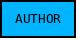
\includegraphics{images/entity.jpeg}}
     & Ορθογώνια: οντότητες. \\ \hline

     \vspace{0.3cm}
     \resizebox*{0.20\textwidth}{!}{
     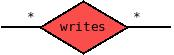
\includegraphics{images/relationship.jpeg}}
     & Ρόμβοι: συσχετίσεις. \\ \hline

     \vspace{0.3cm}
     \resizebox*{0.20\textwidth}{!}{
     
\includegraphics{images/line.jpeg}}
     & Γραμμές: συνδέουν χαρακτηριστικά με οντότητες, οντότητες με συσχετίσεις. \\ \hline

     \vspace{0.3cm}
     %\resizebox*{0.20\textwidth}{!}{
     \center
     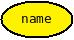
\includegraphics{images/characteristicl.jpeg}%}
     & Ελλείψεις: χαρακτηριστικά. \\ \hline

     \vspace{0.3cm}
     \resizebox*{0.20\textwidth}{!}{
     
\includegraphics{images/characteristicl_many.jpeg}}
     & Διπλές ελλείψεις: πλειότιμα χαρακτηριστικά. \\ \hline

%     \vspace{0.3cm}
     %\resizebox*{0.20\textwidth}{!}{
     \center
%     
\includegraphics{images/characteristicl_many.jpeg}}
%     & Διακεκομμένες ελλείψεις: εξαρτημένα χαρακτηριστικά. \\ \hline

     \vspace{0.3cm}
     %\resizebox*{0.20\textwidth}{!}{
     \center
     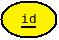
\includegraphics{images/key.jpeg}%}
     & Υπογραμμίσεις: πρωτεύοντα κλειδιά. \\ \hline

     \vspace{0.3cm}
     \resizebox*{0.20\textwidth}{!}{
     
\includegraphics{images/entity_weak.jpeg}}
     & Διπλό ορθογώνιο: Αδύναμο σύνολο οντοτήτων. \\ \hline

     \vspace{0.3cm}
     \resizebox*{0.20\textwidth}{!}{
     
\includegraphics{images/isa.jpeg}}
     & Τρίγωνο: Εξιδίκευση. \\ \hline
  \end{tabular}
\caption{Τα εικονίδια του διαγράμματος οντοτήτων συσχετίσεων.}
\label{table:icons}
\end{center}
\end{table}


%\begin{landscape}
\begin{figure}
\begin{center}
\resizebox*{!}{\textwidth}{
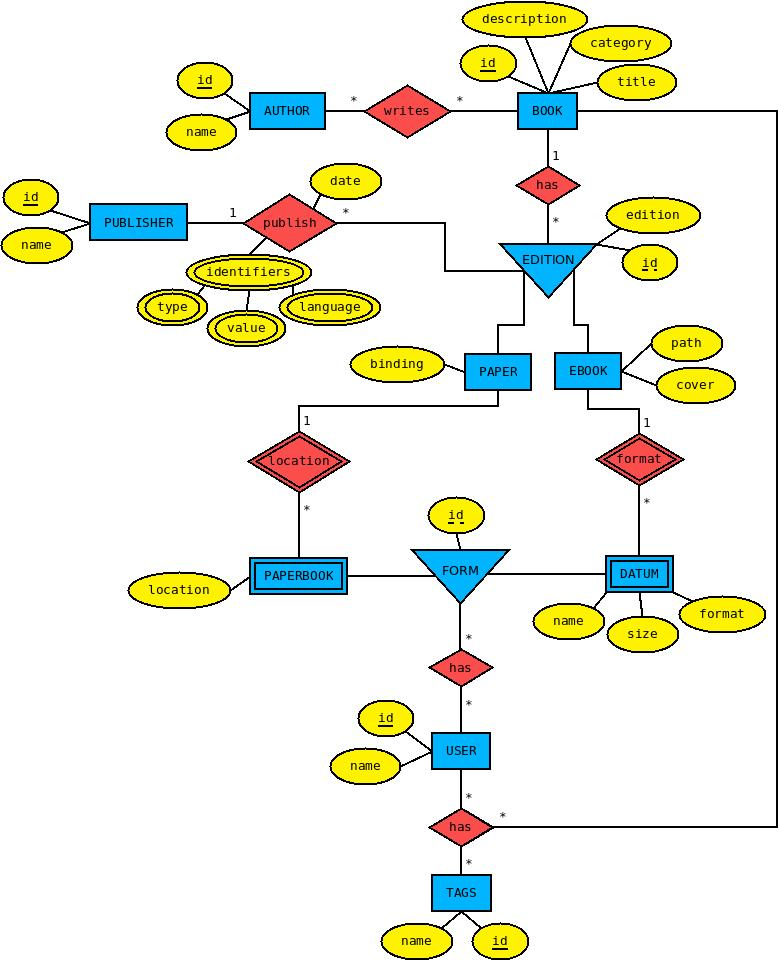
\includegraphics{images/ERDiagram.jpeg}}
\caption{Διάγραμμα οντοτήτων - συσχετίσεων}
\label{fig:ER:diagram}
\end{center}
\end{figure}
%\end{landscape}


Εδώ θα μπει το σχεσιακό μοντέλο της βάσεις που προκύπτει από το μοντέλο οντοτήτων - συσχετίσεων.

Ο λογικός σχεδιασμός είναι η διαδικασία μετατροπής ενός εννοιολογικού μοντέλου (διαισθητικής περιγραφής) σε τυπικά σχήματα εκφρασμένα στο επιλεγέν (υποστηριζόμενο από το ΣΔΒΔ) μοντέλο δεδομένο (π.χ. Σχεσιακό μοντέλο) \cite{class_notes}.

\subsection{Μετατροπή μοντέλου οντοτήτων - συσχετίσεων σε σχεσιακό σχήμα}

Οι κανόνες που χρησιμοποιούνται για την μετατροπή του μοντέλου οντοτήτων - συσχετίσεων σε σχεσιακό σχήμα φαίνονται παρακάτω \cite{class_notes}:

\begin{description}

  \item[Οντότητες:] Ένα ισχυρό σύνολο οντοτήτων μετατρέπεται σε πίνακα (με τα ίδια χαρακτηριστικά). Ένα αδύναμο σύνολο οντοτήτων γίνεται πίνακας που περιλαμβάνει μια στήλη για το πρωτεύον κλειδί του ισχυρότερου συνόλου οντοτήτων που το ταυτοποιεί. 
  \item[Συσχετίσεις 1:1 :] Οι συσχετίσεις 1:1 μπορούν να αναπαρασταθούν είτε προσθέτοντας το πρωτεύον κλειδί της μία πλευράς ως επιπλέον χαρακτηριστικό στον πίνακα της άλλη πλευράς είτε να δημιουργηθεί νέος πίνακας που να έχει τα κλειδιά των δύο πινάκων.
  \item[Συσχετίσεις 1:Ν :] Οι συσχετίσεις 1:Ν μπορούν να αναπαρασταθούν απλά με την προσθήκη ενός επιπλέον χαρακτηριστικού στην πλευρά Ν, με το πρωτεύον κλειδί τις πλευράς 1. Εάν η συμμετοχή στην πλευρά Ν είναι μερική, μπορεί να προκύψει η περίπτωση μία στήλη του πίνακα να έχει πολλές κενές τιμές. Οπότε η δημιουργία ενός νέου πίνακα συμφέρει.
  \item[Συσχετίσεις Μ:Ν :] Ένα σύνολο συσχετίσεων M:N αναπαριστάται ως πίνακας με στήλες για τα πρωτεύοντα κλειδιά των οντοτήτων που συμμετέχουν, και επιπλέον όλα τα χαρακτηριστικά του συνόλου συσχετίσεων. 
  \item[Σύνθετα χαρακτηριστικά :] Τα σύνθετα χαρακτηριστικά μετατρέπονται σε ένα σύνολο απλών.
  \item[Πλειότιμα χαρακτηριστικά :] Από τα πλειότιμα χαρακτηριστικά ενός συνόλου οντοτήτων προκύπτει νέος πίνακας. Ο πίνακας αυτός έχεις ως στήλες το πρωτεύον κλειδί του συνόλου οντοτήτων και μία ακόμα που αντιστοιχεί στο πλειότιμο χαρακτηριστικό.
  \item[Εξειδίκευση :] Όταν έχουμε εξειδίκευση, τότε προκύπτει ένας πίνακας για κάθε εμπλεκόμενο σύνολο οντοτήτων, όπου καθένας από τους πίνακες εξειδίκευσης συμπεριλαμβάνει ως στήλη το πρωτεύον κλειδί του πίνακα γενίκευσης.
 
\end{description}

\begin{landscape}
\begin{figure}
\begin{center}
\resizebox*{23.5cm}{!}{
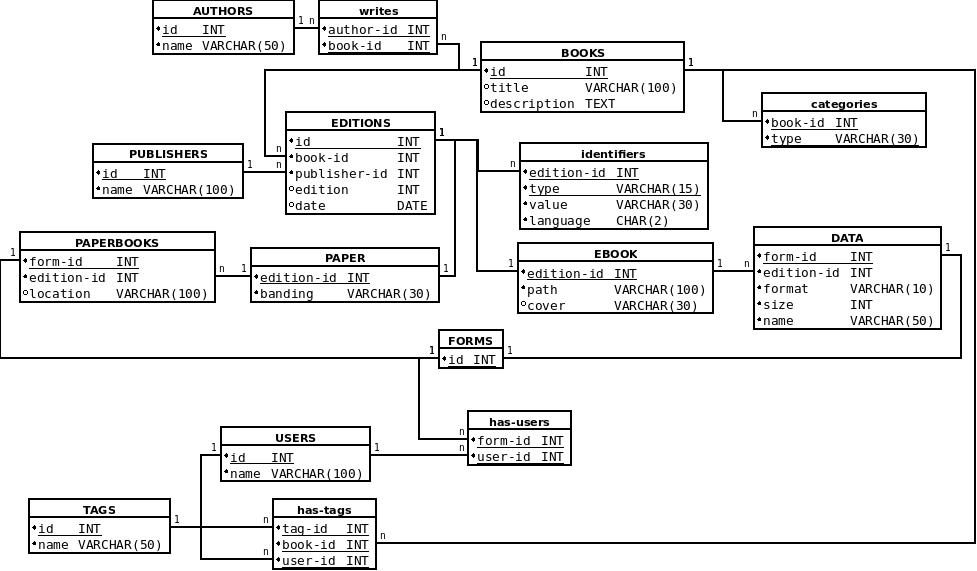
\includegraphics{images/RelationalModel.jpeg}}
\caption{Σχεσιακό σχήμα}
\label{fig:RelationalModel:diagram}
\end{center}
\end{figure}
\end{landscape}


\begin{landscape}
\subsubsection{Ανάλυση πινάκων}


\begin{table}[htbp]
\begin{center}
  \begin{tabular}{|c|c|m{0.35\textwidth}|m{0.35\textwidth}|m{2.0cm}|c|m{1.5cm}|}
    \hline
    {\bf Πεδίο} & {\bf Τύπος μεταβλητής} & {\bf Εύρος τιμών} & {\bf Περιγραφή} & {\bf Πρωτεύον κλειδί} & {\bf Null} & {\bf Ξένο κλειδί} \\ \hline
    id & INT UNSIGNED & 0 έως 4294967295 & Μοναδικός αριθμός που χρησιμεύει ως πρωτεύον κλειδί & ΝΑΙ & ΟΧΙ & ΟΧΙ \\ \hline
    title & VARCHAR(100) & Όλα τα Αλφαριθμητικά ως 100 χαρακτήρες & Ο τίτλος του βιβλίου & ΟΧΙ & ΟΧΙ & ΟΧΙ \\ \hline
    descritpion & TEXT & Όλα τα Αλφαριθμητικά & Μία περιγραφή του βιβλίου & ΟΧΙ & ΟΧΙ & ΟΧΙ \\ \hline
  \end{tabular}
\caption{Ο πίνακας books.}
\label{table:db_table:books}
\end{center}
\end{table}
%\end{landscape}


%\begin{landscape}
\begin{table}[htbp]
\begin{center}
  \begin{tabular}{|c|c|m{0.35\textwidth}|m{0.35\textwidth}|m{2.0cm}|c|m{1.5cm}|}
    \hline
    {\bf Πεδίο} & {\bf Τύπος μεταβλητής} & {\bf Εύρος τιμών} & {\bf Περιγραφή} & {\bf Πρωτεύον κλειδί} & {\bf Null} & {\bf Ξένο κλειδί} \\ \hline
    book-id & INT UNSIGNED & 0 έως 4294967295 & Ξένο κλειδί του πίνακα. Χρησιμοποιείται για την υλοποίηση μίας 1:1 σχέσης με τον πίνακα books & OXI & ΟΧΙ & NAI \\ \hline
  \end{tabular}
\caption{Ο πίνακας paper.}
\label{table:db_table:paper}
\end{center}
\end{table}
\end{landscape}

\begin{landscape}
\begin{table}[htbp]
\begin{center}
  \begin{tabular}{|c|c|m{0.35\textwidth}|m{0.35\textwidth}|m{2.0cm}|c|m{1.5cm}|}
    \hline
    {\bf Πεδίο} & {\bf Τύπος μεταβλητής} & {\bf Εύρος τιμών} & {\bf Περιγραφή} & {\bf Πρωτεύον κλειδί} & {\bf Null} & {\bf Ξένο κλειδί} \\ \hline
    id & INT UNSIGNED & 0 έως 4294967295 & Μοναδικός αριθμός που χρησιμεύει ως πρωτεύον κλειδί & ΝΑΙ & ΟΧΙ & ΟΧΙ \\ \hline
    book-id & INT UNSIGNED & 0 έως 4294967295 & Ξένο κλειδί του πίνακα. Χρησιμοποιείται για την υλοποίηση μίας 1:Ν σχέσης με τον πίνακα books & OXI & ΟΧΙ & NAI \\ \hline
    location & VARCHAR(100) &  Όλα τα Αλφαριθμητικά ως 100 χαρακτήρες & Πεδίο που περιγράφει την φυσική τοποθεσία του βιβλίου & OXI & ΟΧΙ & ΟΧΙ \\ \hline
  \end{tabular}
\caption{Ο πίνακας paperbook.}
\label{table:db_table:paperbook}
\end{center}
\end{table}
\end{landscape}

\begin{landscape}
\begin{table}[htbp]
\begin{center}
  \begin{tabular}{|c|c|m{0.35\textwidth}|m{0.35\textwidth}|m{2.0cm}|c|m{1.5cm}|}
    \hline
    {\bf Πεδίο} & {\bf Τύπος μεταβλητής} & {\bf Εύρος τιμών} & {\bf Περιγραφή} & {\bf Πρωτεύον κλειδί} & {\bf Null} & {\bf Ξένο κλειδί} \\ \hline
    book-id & INT UNSIGNED & 0 έως 4294967295 & Ξένο κλειδί του πίνακα. Χρησιμοποιείται για την υλοποίηση μίας 1:1 σχέσης με τον πίνακα books & OXI & ΟΧΙ & NAI \\ \hline
    path & VARCHAR(100) &  Όλα τα Αλφαριθμητικά ως 100 χαρακτήρες & Το path στο οποίο είναι αποθηκευμένα τα αρχεία των ηλεκτρονικών βιβλίων & OXI & ΟΧΙ & ΟΧΙ \\ \hline
    cover & VARCHAR(100) &  Όλα τα Αλφαριθμητικά ως 100 χαρακτήρες & Το path στο οποίο είναι αποθηκευμένο το εξώφυλλο των ηλεκτρονικών βιβλίων & OXI & ΟΧΙ & ΟΧΙ \\ \hline
  \end{tabular}
\caption{Ο πίνακας ebook.}
\label{table:db_table:ebook}
\end{center}
\end{table}
\end{landscape}

\begin{landscape}
\begin{table}[htbp]
\begin{center}
  \begin{tabular}{|c|c|m{0.35\textwidth}|m{0.35\textwidth}|m{2.0cm}|c|m{1.5cm}|}
    \hline
    {\bf Πεδίο} & {\bf Τύπος μεταβλητής} & {\bf Εύρος τιμών} & {\bf Περιγραφή} & {\bf Πρωτεύον κλειδί} & {\bf Null} & {\bf Ξένο κλειδί} \\ \hline
    id & INT UNSIGNED & 0 έως 4294967295 & Μοναδικός αριθμός που χρησιμεύει ως πρωτεύον κλειδί & ΝΑΙ & ΟΧΙ & ΟΧΙ \\ \hline
    book-id & INT UNSIGNED & 0 έως 4294967295 & Ξένο κλειδί του πίνακα. Χρησιμοποιείται για την υλοποίηση μίας 1:Ν σχέσης με τον πίνακα books & OXI & ΟΧΙ & NAI \\ \hline
    format & VARCHAR(10) &  Όλα τα Αλφαριθμητικά ως 100 χαρακτήρες & Πεδίο που περιγράφει το format του ηλεκτρονικού βιβλίου & OXI & ΟΧΙ & ΟΧΙ \\ \hline
    size & INT UNSIGNED & 0 έως 4294967295 & Πεδίο που περιγράφει το μέγεθος του ηλεκτρονικού βιβλίου σε bytes & OXI & ΟΧΙ & ΟΧΙ \\ \hline
    name & VARCHAR(10) &  Όλα τα Αλφαριθμητικά ως 100 χαρακτήρες & Πεδίο που περιγράφει το όνομα του αρχείου του ηλεκτρονικού βιβλίου & OXI & ΟΧΙ & ΟΧΙ \\ \hline
  \end{tabular}
\caption{Ο πίνακας data.}
\label{table:db_table:data}
\end{center}
\end{table}
\end{landscape}

\begin{landscape}
\begin{table}[htbp]
\begin{center}
  \begin{tabular}{|c|c|m{0.35\textwidth}|m{0.35\textwidth}|m{2.0cm}|c|m{1.5cm}|}
    \hline
    {\bf Πεδίο} & {\bf Τύπος μεταβλητής} & {\bf Εύρος τιμών} & {\bf Περιγραφή} & {\bf Πρωτεύον κλειδί} & {\bf Null} & {\bf Ξένο κλειδί} \\ \hline
    book-id & INT UNSIGNED & 0 έως 4294967295 & Ξένο κλειδί του πίνακα. Χρησιμοποιείται για την υλοποίηση μίας 1:Μ σχέσης με τον πίνακα books & OXI & ΟΧΙ & NAI \\ \hline
    type & VARCHAR(10) & Όλα τα Αλφαριθμητικά ως 10 χαρακτήρες & Περιγράφει το είδος του αναγνωριστικού του βιβλίου (ISBN, amazon id, κ.λ.π.)  & OXI & ΟΧΙ & ΟΧΙ \\ \hline
    type & VARCHAR(20) & Όλα τα Αλφαριθμητικά ως 20 χαρακτήρες & Η τιμή του αναγνωριστικού  & OXI & ΟΧΙ & ΟΧΙ \\ \hline
    language & VARCHAR(2) & Όλα τα Αλφαριθμητικά ως 2 χαρακτήρες & Συντομογραφία της γλώσσας στην οποία είναι γραμμένο το βιβλίο  & OXI & ΟΧΙ & ΟΧΙ \\ \hline
  \end{tabular}
\caption{Ο πίνακας identifiers.}
\label{table::db_table:identifiers}
\end{center}
\end{table}
\end{landscape}

\begin{landscape}
\begin{table}[htbp]
\begin{center}
  \begin{tabular}{|c|c|m{0.35\textwidth}|m{0.35\textwidth}|m{2.0cm}|c|m{1.5cm}|}
    \hline
    {\bf Πεδίο} & {\bf Τύπος μεταβλητής} & {\bf Εύρος τιμών} & {\bf Περιγραφή} & {\bf Πρωτεύον κλειδί} & {\bf Null} & {\bf Ξένο κλειδί} \\ \hline
    id & INT UNSIGNED & 0 έως 4294967295 & Μοναδικός αριθμός που χρησιμεύει ως πρωτεύον κλειδί & ΝΑΙ & ΟΧΙ & ΟΧΙ \\ \hline
    name & VARCHAR(100) & Όλα τα Αλφαριθμητικά ως 100 χαρακτήρες & Ο τίτλος του εκδότη & ΟΧΙ & ΟΧΙ & ΟΧΙ \\ \hline
  \end{tabular}
\caption{Ο πίνακας publishers.}
\label{table:db_table:publishers}
\end{center}
\end{table}
%\end{landscape}

%\begin{landscape}
\begin{table}[htbp]
\begin{center}
  \begin{tabular}{|c|c|m{0.35\textwidth}|m{0.35\textwidth}|m{2.0cm}|c|m{1.5cm}|}
    \hline
    {\bf Πεδίο} & {\bf Τύπος μεταβλητής} & {\bf Εύρος τιμών} & {\bf Περιγραφή} & {\bf Πρωτεύον κλειδί} & {\bf Null} & {\bf Ξένο κλειδί} \\ \hline
    publisher-id & INT UNSIGNED & 0 έως 4294967295 & Ξένο κλειδί του πίνακα. Χρησιμοποιείται για την υλοποίηση μίας 1:Μ σχέσης με τον πίνακα publishers & OXI & ΟΧΙ & NAI \\ \hline
    book-id & INT UNSIGNED & 0 έως 4294967295 & Ξένο κλειδί του πίνακα. Χρησιμοποιείται για την υλοποίηση μίας 1:Μ σχέσης με τον πίνακα books & OXI & ΟΧΙ & NAI \\ \hline
    date & DATE & 1000-01-01 έως 9999-12-31 & Ημερομηνία έκδοσης του βιβλίου & OXI & ΟΧΙ & ΟΧΙ \\ \hline
  \end{tabular}
\caption{Ο πίνακας publish.}
\label{table:db_table:publish}
\end{center}
\end{table}
\end{landscape}

\begin{landscape}
\begin{table}[htbp]
\begin{center}
  \begin{tabular}{|c|c|m{0.35\textwidth}|m{0.35\textwidth}|m{2.0cm}|c|m{1.5cm}|}
    \hline
    {\bf Πεδίο} & {\bf Τύπος μεταβλητής} & {\bf Εύρος τιμών} & {\bf Περιγραφή} & {\bf Πρωτεύον κλειδί} & {\bf Null} & {\bf Ξένο κλειδί} \\ \hline
    id & INT UNSIGNED & 0 έως 4294967295 & Μοναδικός αριθμός που χρησιμεύει ως πρωτεύον κλειδί & ΝΑΙ & ΟΧΙ & ΟΧΙ \\ \hline
    name & VARCHAR(100) & Όλα τα Αλφαριθμητικά ως 100 χαρακτήρες & Το όνομα του συγγραφέα & ΟΧΙ & ΟΧΙ & ΟΧΙ \\ \hline
  \end{tabular}
\caption{Ο πίνακας authors.}
\label{table:db_table:authors}
\end{center}
\end{table}
%\end{landscape}

%\begin{landscape}
\begin{table}[htbp]
\begin{center}
  \begin{tabular}{|c|c|m{0.35\textwidth}|m{0.35\textwidth}|m{2.0cm}|c|m{1.5cm}|}
    \hline
    {\bf Πεδίο} & {\bf Τύπος μεταβλητής} & {\bf Εύρος τιμών} & {\bf Περιγραφή} & {\bf Πρωτεύον κλειδί} & {\bf Null} & {\bf Ξένο κλειδί} \\ \hline
    author-id & INT UNSIGNED & 0 έως 4294967295 & Ξένο κλειδί του πίνακα. Χρησιμοποιείται για την υλοποίηση μίας 1:Μ σχέσης με τον πίνακα authors & OXI & ΟΧΙ & NAI \\ \hline
    book-id & INT UNSIGNED & 0 έως 4294967295 & Ξένο κλειδί του πίνακα. Χρησιμοποιείται για την υλοποίηση μίας 1:Μ σχέσης με τον πίνακα books & OXI & ΟΧΙ & NAI \\ \hline
  \end{tabular}
\caption{Ο πίνακας writes.}
\label{table:db_table:writes}
\end{center}
\end{table}
\end{landscape}

\begin{landscape}
\begin{table}[htbp]
\begin{center}
  \begin{tabular}{|c|c|m{0.35\textwidth}|m{0.35\textwidth}|m{2.0cm}|c|m{1.5cm}|}
    \hline
    {\bf Πεδίο} & {\bf Τύπος μεταβλητής} & {\bf Εύρος τιμών} & {\bf Περιγραφή} & {\bf Πρωτεύον κλειδί} & {\bf Null} & {\bf Ξένο κλειδί} \\ \hline
    id & INT UNSIGNED & 0 έως 4294967295 & Μοναδικός αριθμός που χρησιμεύει ως πρωτεύον κλειδί & ΝΑΙ & ΟΧΙ & ΟΧΙ \\ \hline
    name & VARCHAR(100) & Όλα τα Αλφαριθμητικά ως 100 χαρακτήρες & Το όνομα του χρήστη & ΟΧΙ & ΟΧΙ & ΟΧΙ \\ \hline
  \end{tabular}
\caption{Ο πίνακας users.}
\label{table:db_table:users}
\end{center}
\end{table}
%\end{landscape}

%\begin{landscape}
\begin{table}[htbp]
\begin{center}
  \begin{tabular}{|c|c|m{0.35\textwidth}|m{0.35\textwidth}|m{2.0cm}|c|m{1.5cm}|}
    \hline
    {\bf Πεδίο} & {\bf Τύπος μεταβλητής} & {\bf Εύρος τιμών} & {\bf Περιγραφή} & {\bf Πρωτεύον κλειδί} & {\bf Null} & {\bf Ξένο κλειδί} \\ \hline
    book-id & INT UNSIGNED & 0 έως 4294967295 & Ξένο κλειδί του πίνακα. Χρησιμοποιείται για την υλοποίηση μίας 1:Μ σχέσης με τον πίνακα books & OXI & ΟΧΙ & NAI \\ \hline
    user-id & INT UNSIGNED & 0 έως 4294967295 & Ξένο κλειδί του πίνακα. Χρησιμοποιείται για την υλοποίηση μίας 1:Μ σχέσης με τον πίνακα users & OXI & ΟΧΙ & NAI \\ \hline
  \end{tabular}
\caption{Ο πίνακας has-users.}
\label{table:db_table:has-users}
\end{center}
\end{table}
\end{landscape}

\begin{landscape}
\begin{table}[htbp]
\begin{center}
  \begin{tabular}{|c|c|m{0.35\textwidth}|m{0.35\textwidth}|m{2.0cm}|c|m{1.5cm}|}
    \hline
    {\bf Πεδίο} & {\bf Τύπος μεταβλητής} & {\bf Εύρος τιμών} & {\bf Περιγραφή} & {\bf Πρωτεύον κλειδί} & {\bf Null} & {\bf Ξένο κλειδί} \\ \hline
    id & INT UNSIGNED & 0 έως 4294967295 & Μοναδικός αριθμός που χρησιμεύει ως πρωτεύον κλειδί & ΝΑΙ & ΟΧΙ & ΟΧΙ \\ \hline
    name & VARCHAR(100) & Όλα τα Αλφαριθμητικά ως 100 χαρακτήρες & Το όνομα του tag & ΟΧΙ & ΟΧΙ & ΟΧΙ \\ \hline
  \end{tabular}
\caption{Ο πίνακας tags.}
\label{table:db_table:tags}
\end{center}
\end{table}
\end{landscape}

\begin{landscape}
\begin{table}[htbp]
\begin{center}
  \begin{tabular}{|c|c|m{0.35\textwidth}|m{0.35\textwidth}|m{2.0cm}|c|m{1.5cm}|}
    \hline
    {\bf Πεδίο} & {\bf Τύπος μεταβλητής} & {\bf Εύρος τιμών} & {\bf Περιγραφή} & {\bf Πρωτεύον κλειδί} & {\bf Null} & {\bf Ξένο κλειδί} \\ \hline
    tag-id & INT UNSIGNED & 0 έως 4294967295 & Ξένο κλειδί του πίνακα. Χρησιμοποιείται για την υλοποίηση μίας 1:Μ σχέσης με τον πίνακα tags & OXI & ΟΧΙ & NAI \\ \hline
    book-id & INT UNSIGNED & 0 έως 4294967295 & Ξένο κλειδί του πίνακα. Χρησιμοποιείται για την υλοποίηση μίας 1:Μ σχέσης με τον πίνακα books & OXI & ΟΧΙ & NAI \\ \hline
    user-id & INT UNSIGNED & 0 έως 4294967295 & Ξένο κλειδί του πίνακα. Χρησιμοποιείται για την υλοποίηση μίας 1:Μ σχέσης με τον πίνακα users & OXI & ΟΧΙ & NAI \\ \hline
  \end{tabular}
\caption{Ο πίνακας has-tags.}
\label{table:db_table:has-tags}
\end{center}
\end{table}
\end{landscape}

\subsection{Υλοποίηση}



\begin{minted}{bash}
$ mysql --user=root --password
Enter password: 
\end{minted} 

%%$

\begin{minted}[breaklines=true]{mysql}
MariaDB [(none)]> CREATE USER 'book'@'localhost' IDENTIFIED BY 'book_password' ;

MariaDB [(none)]> GRANT USAGE ON *.* TO 'book'@'localhost' IDENTIFIED BY 'book_password' WITH MAX_QUERIES_PER_HOUR 0 MAX_CONNECTIONS_PER_HOUR 0 MAX_UPDATES_PER_HOUR 0 MAX_USER_CONNECTIONS 0 ;

MariaDB [(none)]> CREATE DATABASE `book` ;

MariaDB [(none)]> GRANT ALL PRIVILEGES ON `book`.* TO 'book'@'localhost';

\end{minted}

\begin{minted}{bash}
$ mysql --user=book --password
Enter password: 
\end{minted} 

%%$

\begin{minted}[breaklines=true]{mysql}
MariaDB [(none)]> show databases;
+--------------------+
| Database           |
+--------------------+
| information_schema |
| book               |
+--------------------+
2 rows in set (0.00 sec)

MariaDB [(none)]> use book;
Database changed
MariaDB [book]> 

\end{minted}

\begin{minted}[breaklines=true]{mysql}
MariaDB [book]> CREATE TABLE books (
    -> id INT UNSIGNED NOT NULL AUTO_INCREMENT,
    -> title VARCHAR(100) NOT NULL,
    -> description TEXT NOT NULL,
    -> PRIMARY KEY (id) );
Query OK, 0 rows affected (0.15 sec)

MariaDB [book]> describe BOOKS;
+-------------+------------------+------+-----+---------+----------------+
| Field       | Type             | Null | Key | Default | Extra          |
+-------------+------------------+------+-----+---------+----------------+
| id          | int(10) unsigned | NO   | PRI | NULL    | auto_increment |
| title       | varchar(100)     | NO   |     | NULL    |                |
| description | text             | NO   |     | NULL    |                |
+-------------+------------------+------+-----+---------+----------------+
3 rows in set (0.00 sec)


\end{minted}

\begin{minted}[breaklines=true]{mysql}
MariaDB [book]> CREATE TABLE identifiers (
    -> book_id INT UNSIGNED NOT NULL, 
    -> type VARCHAR(50) NOT NULL, 
    -> value VARCHAR(50) NOT NULL, 
    -> language CHAR(2) NOT NULL, 
    -> FOREIGN KEY (book_id) REFERENCES BOOKS(id) );
Query OK, 0 rows affected (0.07 sec)


MariaDB [book]> describe identifiers;
+----------+------------------+------+-----+---------+-------+
| Field    | Type             | Null | Key | Default | Extra |
+----------+------------------+------+-----+---------+-------+
| book_id  | int(10) unsigned | NO   | MUL | NULL    |       |
| type     | varchar(50)      | NO   |     | NULL    |       |
| value    | varchar(50)      | NO   |     | NULL    |       |
| language | char(2)          | NO   |     | NULL    |       |
+----------+------------------+------+-----+---------+-------+
4 rows in set (0.00 sec)

\end{minted}

\phantomsection \label{Βιβλιογραφία}
\addcontentsline{toc}{section}{Βιβλιογραφία}
%\mtcaddchapter[Βιβλιογραφία] % Λόγω του minitoc
\bibliographystyle{plain}
\bibliography{references}

\newpage

\end{document}

